%
% chapter.tex -- Kapitel über Multiskalen-Analyse
%
% (c) 2019 Prof Dr Andreas Müller, Hochschule Rapperswil
%
\chapter{Multiskalen-Analyse
\label{chapter:msa}}
\lhead{Multiskalen-Analyse}
Die Funktionen $\psi_{a,b}(t)$ der stetigen Wavelet-Transformation
sind in hohem Masse redundant.
Ausserdem muss man sich beim praktischen Einsatz auf diskretisierte 
Versionen beschränken, man muss also eine Auswahl unter den möglichen
Werten $(a,b)$ treffen.
Wie muss diese Auswahl erfolgen, damit eine Theorie resultiert, die
immer noch alle Symmetrien hat, die man zum Beispiel beim Haar-Servlet
gefunden hat?
In diesem Kapitel wird das Konzept der Multi-Skalen-Analyse vorgestellt.
Sie fasst viele der bisher entwickelten Ideen in einem abstrakten
Rahmen zusammen und ermöglicht damit, allgemeine Vorgehensweisen für die
Konstruktion einer Waveletbasis zu formulieren.
Im Kapitel~\ref{chapter:algo} werden daraus die schnellen numerischen
Algorithmen für die Wavelet-Transformation abgeleitet.

%
% defintion.tex -- MSA definition
%
% (c) 2019 Prof Dr Andreas Müller
%
\section{Skalen und Vektorräume
\label{section:skalen und vektorraeume}}
\rhead{Skalen und Vektorräume}

\subsection{Ein Turm von Vektorräumen}
Wir möchten zum Ausdruck bringen, dass Funktionen in $L^2(\mathbb R)$
mit zunehmender Genauigkeit approximiert werden können durch Funktionen,
die immer mehr Einzelheiten auflösen.
Sei also $V_0\subset L^2(\mathbb R)$ eine Menge von Funktionen, wobei wir
uns vorstellen, dass darin Funktionsdetails bis zur Länge eins aufgelöst
sind.
Im Beispiel des Haar-Wavelets wäre der Raum der Funktionen, die
zwischen ganzzahligen $t$-Werten konstant sind, ein geeigneter Raum,
der diese Intuition wiedergibt.

Wir erwarten, dass $V_0$ dazu geeignet ist, Funktionen aus $L^2$ auf
eine translationsinvariante Art zu approximieren.
Das geht aber nur, wenn mit $f\in V_0$ auch alle verschobenen Funktionen
$T_bf\in V_0$ sind für $b\in\mathbb Z$.

Durch Skalierung von Funktionen wird es möglich werden, weitere Details
aufzulösen.
Der Vektorraum $V_j$ soll die Menge der Funktionen umfassen, die Details
bis zur Grösse $2^{-j}$ darstellen kann.
Im Haar-Wavelet-Beispiel sind das die Funktionen, die zwischen Punkten
konstant sind, die ganzzahlige Vielfache von $2^{-j}$ sind.
Je mehr Details aufgelöst werden können, desto grösser sind die
Vektorräume.
Es entsteht ein Turm
\begin{equation}
\dots
V_{-2}\subset
V_{-1}\subset
V_0\subset
V_1\subset
V_2\subset
\dots
V_j\subset
\dots
\subset L^2(\mathbb R)
\label{buch:skalen-turm}
\end{equation}
von Unterräumen von $L^2(\mathbb R)$.

Der Turm~\eqref{buch:skalen-turm} drückt noch nicht aus, dass die
Funktionen, die höhere Details wiedergeben, skalierte Versionen der
``gröberen'' Funktionen sind.
Daher wird gefordert, dass
\[
f\in V_j \quad\Rightarrow\quad D_2f\in V_{j+1}
\qquad\text{oder}\qquad
D_2V_j \subset V_{j+1}
\]
Dies drückt aber noch nicht aus, dass in $V_{j+1}$ noch mehr Details
aufgelöst werden können, als mit Hilfe von skalierten Versionen der
Funktionen in $V_j$ möglich ist.
Dazu muss verlangt werden, dass
$D_2V_j = V_{j+1}$
gilt.

Es wäre zu viel verlangt, dass jede Funktion in $L^2(\mathbb R)$ in
einem der Vektorräume $V_j$ liegt, denn in $L^2(\mathbb R)$ gibt
es ja einige ``ganz verrückte'' Funktionen.
Die Abtastung soll also detailliert genug sein, dass jede 
Funktion in $L^2(\mathbb R)$ beliebig genau durch Funktionen aus
der Vereinigung aller $V_j$ approximiert werden kann.
Dies wird durch
\[
\overline{\bigcup_{j\in Z} V_j} = L^2(\mathbb R)
\]
ausgedrückt, wobei der Querstrich den Abschluss, die Menge aller Grenzwerte
von Folgen der Vereinigung der $V_j$ bezeichnet.

Wird die Auflösung schrittweise reduziert, dann bleibt nur die Nullfunktion
übrig.
Es gibt also keine Funktionen mit Features, die beliebig weit ausgedehnt
sind im Sinne der Vektorräume $V_j$.
Man kann dies durch
\[
\bigcap_{j\in\mathbb Z} V_j = \{0\}
\]
ausdrücken.

Damit haben wir alle Elemente zusammen für die formale Definition.

\begin{definition}
Eine {\em Multiskalen-Analyse} ist ein Turm
\[
\dots
V_{-2}\subset
V_{-1}\subset
V_0\subset
V_1\subset
V_2\subset
\dots
V_j\subset
\dots
\]
von Unterräumen von $L^2(\mathbb R)$
mit den folgenden Eigenschaften
\begin{enumerate}
\item $\bigcap_{j\in\mathbb Z} V_j = \{0\}$
\item $\overline{\bigcup_{j\in\mathbb Z} V_j} = L^2(\mathbb R)$.
\item Es gibt eine Funktion $\psi\in V_0$ derart, dass
die Translate $T_b\psi$ mit $b\in\mathbb Z$ den Raum $W_0$ erzeugen:
\[
W_0 = \overline{\langle T_b\psi\;|\;b\in\mathbb Z\rangle}.
\]
\end{enumerate}
\end{definition}

\begin{figure}
\centering
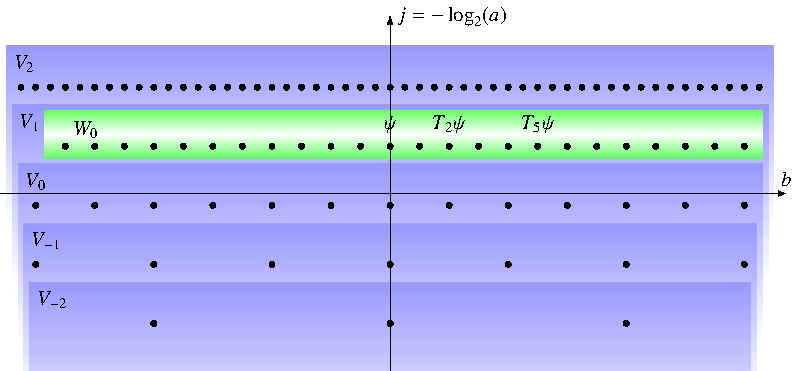
\includegraphics{chapters/6-msa/images/msa.pdf}
\caption{Hierarchie der Vektorräume $V_j$ sowie der Komplemente $W_j$
mit
$V_{j+1} = V_j \oplus = W_j$.
\label{msa:vektorraumhierarchie}}
\end{figure}

Man beachte, es wird nicht verlangt, dass die $T_b\psi$ orthogonal
sein müssen.

\begin{beispiel}
Das Haar-Wavelet erzeugt eine Multiskalen-Analyse von $L^2(\mathbb R)$.
% XXX TODO Haar MRA darstellen
\end{beispiel}

\begin{beispiel}
% XXX TODO MRA der auf 2-adischen Intervallen stückweise linearen Funktionen
\end{beispiel}

\subsection{Orthogonalität}

% XXX TODO Kette von Vektorräumen
% XXX TODO V_j und W_j
% XXX TODO Orthogonalitätseigenschaften
% XXX TODO Projektionsoperatoren

%
% skalfour.tex
%
% (c) 2019 Prof Dr Andreas Müller, Hochschule Rapperswil
%
\section{Skalierungsrelation und Fouriertransformation
\label{section:skalfour}}
\rhead{Skalierungsrelation und Fouriertransformation}

% XXX TODO Funktion H und Skalierungsrelation

Gibt es überhaupt eine Funktion $\varphi$ derart, dass die Translate
$T_b\varphi$ mit $b\ne 0$ alle orthogonal sind?
Lange Zeit war nicht klar, dass es ausser dem schon lange bekannten
Haar-Wavelet tatsächlich solche Funktionen gibt.
Yves Meyer versuchte sogar erst zu zeigen, dass das Haar-Wavelet das
einzige mit dieser Eigenschaft ist.
In diesem Abschnitt untersuchen wir diese Eigenschaft mit Hilfe der 
Fourier-Theorie.
In Abschnitt~\ref{section:orthonormalisierung} werden wir später sehen,
dass sich für fast beliebige Funktionen $f$ eine Linearkombination
$\varphi$ von Translaten von $f$ finden lässt, so dass die Translate
von $\varphi$ orthonormiert sind.

%
% Interval-Trick: Aufteilung eines Fourier-Integrals in Teilintervalle
%                 für ganzzahlige Argumente
%
\subsection{Der Interval-Trick und der Periodisierungs-Operator}
Wir werden im Folgenden wiederholt einen Trick verwenden, mit dem
Fourier-Integrale über $\mathbb R$ in gewöhnliche Integrale
über ein endliches Interval umgeformt werden können.
Sei $f$ eine Funktion auf $\mathbb R$ und $b,\,k\in\mathbb Z$.
Da $b,\,k$ ganze Zahlen sind, ist
\[
e^{ib(t+2\pi k)}
=
e^{ibt}\underbrace{e^{2\pi i bk}}_{\displaystyle = 1}
=
e^{ibt},
\]
da $bk$ ebenfalls eine ganze Zahl ist.
Dann kann man den Integrationsbereich $\mathbb R$ in Intervalle der
Länge $2\pi$ jeweils zwischen $2\pi k$ und $2\pi(k+1)$ aufteilen.
Für das Fourier-Integral folgt dann
\begin{align}
\int_{-\infty}^\infty f(t) e^{-ibt}\,dt
&=
\sum_{k\in\mathbb Z} \int_{2\pi k}^{2\pi(k+1)} f(t) e^{-ibt}\,dt
=
\sum_{k\in\mathbb Z} \int_{0}^{2\pi} f(t+2\pi k) e^{-ibt}\,dt
=
\int_{0}^{2\pi} \biggl(\sum_{k\in\mathbb Z} f(t+2\pi k)\biggr) e^{-ibt}\,dt
\label{msa:intervaltrick}
\end{align}
Der Klammerausdruck ist eine $2\pi$-periodische Funktion auf $\mathbb R$.
Wir werden diese Operation wiederholt benötigen und spendieren ihr daher
eine formelle Definition

\begin{definition}
\label{msa:peri}
Für eine Funktion $f\in L^2(\mathbb R)$ ist die periodisch gemachte Funktion
\[
\mathcal{P}f(t) = \sum_{k\in\mathbb Z} f(t+2\pi k)
\]
eine Funktion $L^2([0,2\pi])$.
$\mathcal{P}$ heisst Periodisierungs-Operator.
\end{definition}
\index{Periodisierungs-Operator}%

\begin{proof}[Beweis]
Die Definition behauptet, dass die Operation $\mathcal{P}$ für
quadratintegrierbare Funktionen auf $\mathbb R$ eine quadratintegrierbare
Funktion $2\pi$-periodische Funktion ergibt.
Wir rechnen dazu nach
\begin{align*}
\int_{0}^{2\pi}
| \mathcal{P}f(t)|^2
\,dt
&=
\int_{0}^{2\pi}
\biggl|
\sum_{k\in\mathbb Z}f(t+2\pi k)
\biggr|^2
\,dt
\\
&\le
\int_{-\infty}^\infty |f(t)|^2 \,dt
=
\| f\|^2.
\qedhere
\end{align*}
\end{proof}

Da $b\in\mathbb Z$, berechnet das Integral~\eqref{msa:intervaltrick}
bis auf einen Faktor $2\pi$ die Fourier-Koeffizienten von $\mathcal{P}f$.
Wir haben daher den folgenden Satz gefunden:

\begin{satz}
\label{msa:Pfourier}
Ist $f\in L^2(\mathbb R)$, dann sind die Fourier-Koeffizienten von
$\mathcal{P}f$
\[
\widehat{\mathcal{P}f}(b)
=
\frac1{2\pi}\int_{0}^{2\pi} \mathcal{P}f(t) e^{-ibt}\,dt
=
\frac1{2\pi}
\int_{-\infty}^\infty f(t) e^{-ibt}\,dt
=
\frac{1}{\sqrt{2\pi}} \hat{f}(b).
\]
\end{satz}

Die Fourier-Koeffizienten der periodisch gemachten Funktion $\mathcal{P}f$ 
hängen also mit den Werten der Fourier-Transformation an ganzzahligen
Punkten zusammen.

\begin{lemma}
Der Periodisierungs-Operator $\mathcal{P}$ ist linear:
\begin{align*}
\mathcal{P}(f+g)(t)
&=
\mathcal{P}f(t) + \mathcal{P}g(t),
\\
\mathcal{P}(\lambda f)(t)
&=
\lambda \mathcal{P}f(t).
\end{align*}
\end{lemma}

\begin{proof}[Beweis]
Diese Identitäten können durch Nachrechnen verifiziert werden:
\begin{align*}
\mathcal{P}(f+g)(t)
&=
\sum_{k\in\mathbb Z}(f+g)(t+2\pi k)
=
\sum_{k\in\mathbb Z}\bigl(f(t+2\pi k)+ g(t+2\pi k)\bigr)
\\
&=
\sum_{k\in\mathbb Z}\bigl(f(t+2\pi k)
+
\sum_{k\in\mathbb Z}g(t+2\pi k)\bigr)
\\
&=
\mathcal{P}f(t)
+
\mathcal{P}g(t),
\\
\mathcal{P}(\lambda f)(t)
&=
\sum_{k\in\mathbb Z}(\lambda f)(t+2\pi k)
=
\sum_{k\in\mathbb Z}\lambda f(t+2\pi k)
=
\lambda
\sum_{k\in\mathbb Z}f(t+2\pi k)
=
\lambda \mathcal{P}f(t).
\qedhere
\end{align*}
\end{proof}

%
% Orthogonalitätsbedingung für die Translate des Vater-Wavelets
%
\subsection{Orthogonalität der Translate von $\varphi$}
Die Funktion $\varphi$ hat die Bedingung zu erfüllen, dass
\[
\langle \varphi, T_b\varphi\rangle = \delta_{b0}
\qquad\forall b\in\mathbb Z.
\]
Wir verwenden die Plancherel-Formel für die Fourier-Transformation,
um dieses Skalarprodukt zu vereinfachen:
\begin{align*}
\langle \varphi,T_b\varphi\rangle
&=
\langle \hat{\varphi},\widehat{T_b\varphi}\rangle
=
\int_{-\infty}^\infty
\hat{\varphi}(\omega) e^{i\omega b}\overline{\hat{\varphi}(\omega)}
\,d\omega
=
\int_{-\infty}^\infty
|\hat{\varphi}(\omega)|^2 e^{i\omega b}
\,d\omega.
\\
\intertext{Dies ist genau ein Integral der Art~\eqref{msa:intervaltrick}.
Wir können es daher durch Fourier-Koeffizienten der periodische 
gemachten Funktion $\mathcal{P}|\hat{\varphi}|^2$ ausdrücken und
erhalten
}
&=
\int_0^{2\pi}
\mathcal{P}|\hat{\varphi}|^2(\omega) e^{-ib\omega}
\,d\omega
=
\int_0^{2\pi}
\biggl(
\sum_{k\in\mathbb Z}
|\hat{\varphi}(\omega + 2\pi k)|^2\biggr)
e^{-i\omega b}
\,d\omega.
\intertext{Die Orthogonalitätsbedingung lautet jetzt}
\langle \varphi,T_b\varphi\rangle
&=
2\pi
\widehat{\mathcal{P}|\hat{\varphi}|^2}(-b)
=
\delta_{0b}.
\end{align*}
\index{Orthgonalitätsbedingung}
Die Funktion $\mathcal{P}|\hat{\varphi}|^2$ ist also $2\pi$-periodisch und
derart, dass alle Fourier-Koeffizienten ausser der Koeffizienten für
$b=0$ verschwinden.
Diese Funktion muss daher eine Konstante sein.
Damit haben wir den folgenden Satz bewiesen.

\begin{satz}
\label{satz:msa:orthogonalitaetsbedingung}
Damit die ganzzahligen Translate einer Funktion $\varphi\in L^2$ alle
orthogonal sind, ist notwendig und hinreichend, dass 
\begin{equation}
\mathcal{P}|\hat{\varphi}|^2(\omega)
=
\sum_{k\in\mathbb Z} |\hat{\varphi}(\omega + 2\pi k)|^2
=
\frac1{2\pi}
\label{msa:orthogonalitaetsbedingung}
\end{equation}
ist für fast alle $\omega\in\mathbb R$.
\end{satz}
\index{Orthogonalitätsbedingung}

Dieselbe Idee lässt sich auch auf Funktionen anwenden, die orthogonal
sind zu allen Translaten.

\begin{satz}
\label{satz:msa:alleorthogonal}
Seien $\varphi,\psi\in L^2$, dann ist $\varphi$ orthogonal zu allen
ganzzahligen Translaten $T_b\psi$  von $\psi$ genau dann, wenn
\begin{equation}
\sum_{k\in\mathbb Z} \hat{\varphi}(\omega+2\pi k)\overline{\hat{\psi}(\omega+2\pi k)}
=
0
\end{equation}
für fast alle $\omega\in\mathbb R$.
\end{satz}

\begin{proof}[Beweis]
Nach Voraussetzung gilt für alle $b\in\mathbb Z$
\begin{align*}
0
&=
\langle \varphi,T_b\psi\rangle
=
\langle \hat{\varphi}, \widehat{T_b\psi}\rangle
=
\int_{-\infty}^\infty
\hat{\varphi}(\omega)\, \overline{\hat{\psi}(\omega)} e^{ib\omega}
\,d\omega
\\
&=
2\pi
\widehat{\mathcal{P}(\hat{\varphi}\bar{\hat{\psi}})}(b)
\end{align*}
Die $2\pi$-periodische Funktion $\mathcal{P}(\hat{\varphi}\bar{\hat{\psi}})$ 
hat also lauter verschwindende Fourier-Koeffizienten, also verschwindet
sie.
Nach Definition ist
\[
\mathcal{P}(\hat{\varphi}\bar{\hat{\psi}})
=
\sum_{k\in\mathbb Z}
\hat{\varphi}(\omega + 2\pi k)
\bar{\hat{\psi}}(\omega + 2\pi k)
=0.
\]
Dies beweist die Aussage.
\end{proof}

%
% Skalierungsrelation
%
\subsection{Die Skalierungsrelation
\label{msa:skal}}
Das Vater-Wavelet einer Multiskalen-Analyse muss einer Skalierungsrelation
genügen, die wir in der Form
\begin{equation}
\varphi(t)
=
\sqrt{2} \sum_{k\in\mathbb Z} h_k \varphi(2t-k)
\label{msa:skalt}
\end{equation}
schreiben.
\index{Skalierungsrelation}
Wir wenden darauf die Fourier-Transformation an und erhalten
\[
\hat{\varphi}(t)
=
\sqrt{2} \sum_{k\in\mathbb Z} h_k e^{-ik\omega/2} \frac12\hat{\varphi}\biggl(\frac{\omega}{2}\biggr)
=
\frac1{\sqrt{2}}
\biggl(\sum_{k\in\mathbb Z}h_ke^{-ik\omega/2}\biggr)
\hat{\varphi}\biggl(\frac{\omega}2\biggr)
\]

\begin{definition}
\label{definition:erzeugende-funktion-msa}
Wir schreiben 
\[
H(s)
=
\frac1{\sqrt{2}}
\sum_{k\in\mathbb Z}h_ke^{-iks},
\]
für die sogenannte {\em erzeugende Funktion} einer Multiskalen-Analyse.
\end{definition}
\index{erzeugende Funktion einer MSA}

Mit der erzeugenden Funktion $H(s)$ wird die
Skalierungsbedingung~\eqref{msa:skalt} im Zeitbereich
für das Vater-Wavelet zu der Bedingung
\begin{equation}
\hat{\varphi}(\omega) 
=
H\biggl(\frac{\omega}2\biggr)\,\hat{\varphi}\biggl(\frac{\omega}2\biggr)
\label{msa:skalomega}
\end{equation}
im Frequenzbereich.
Wir haben in \eqref{msa:skalomega}
also eine zusätzliche Bedingung zur Orthogonalitätsbedingung
\eqref{msa:orthogonalitaetsbedingung}.

Man beachte, dass die Funktion $H(s)$ ausschliesslich durch die
Koeffizienten der Skalierungsrelation bestimmt ist.
Die Funktionalgleichung~\eqref{msa:skalomega} deutet bereits an,
dass diese Koeffizienten die Funktion $\varphi$ eindeutig bestimmen
könnten.

Ein weiterer Schritt in diese Richtung ist, dass sich die
Orthogonalitätsbedingung~\eqref{msa:orthogonalitaetsbedingung}
durch $H$ ausdrücken lässt.

\begin{satz}
\label{satz:Hbed}
Die erzeugende Funktion $H(s)$ einer Multiskalen-Analyse erfüllt die
Bedingung
\begin{equation}
|H(\omega)|^2 + |H(\omega+\pi)|^2 = 1
\label{msa:Hbed}
\end{equation}
für fast alle $\omega\in\mathbb R$.
\end{satz}

\begin{proof}[Beweis]
Wir spalten die Summe in der Orthogonalitätsbedingung in zwei
Teilsummen mit geraden und ungeraden $k$ auf:
\begin{align*}
\frac{1}{2\pi}
&=
\sum_{k\in\mathbb Z} |\hat{\varphi}(\omega + 2\pi k)|^2
=
\sum_{k\in\mathbb Z} |\hat{\varphi}(\omega + 4\pi k)|^2
+
\sum_{k\in\mathbb Z} |\hat{\varphi}(\omega + 4\pi k + 2\pi)|^2
\\
\intertext{und wenden auf jeden Summanden die 
Skalierungsrelation~\eqref{msa:skalomega} an:}
&=
\sum_{k\in\mathbb Z}
\biggl|
H\biggl(\frac{\omega}2+2\pi k\biggr)
\hat\varphi\biggl(\frac{\omega}2 + 2\pi k\biggr)
\biggr|^2
+
\sum_{k\in\mathbb Z}
\biggl|
H\biggl(\frac{\omega}2 + \pi + 2\pi k\biggr)
\hat\varphi\biggl(\frac{\omega}2 + \pi+ 2\pi k\biggr)
\biggr|^2
\\
&=
\biggl|
H\biggl(\frac{\omega}2\biggr)
\biggr|^2
\sum_{k\in\mathbb Z}
\biggl|
\hat\varphi\biggl(\frac{\omega}2 + 2\pi k\biggr)
\biggr|^2
+
\biggl|
H\biggl(\frac{\omega}2 + \pi\biggr)
\biggr|^2
\sum_{k\in\mathbb Z}
\biggl|
\hat\varphi\biggl(\frac{\omega}2 + \pi+ 2\pi k\biggr)
\biggr|^2
\intertext{Darin können wir die Summanden $2\pi k$ in den Argumenten von
$H$ weglassen, weil $H$ $2\pi$-periodisch ist.
$k$ verschwindet damit aus den Faktoren $H$, die daher aus der
Summe ausgeklammert werden können:}
&=
\biggl|
H\biggl(\frac{\omega}2\biggr)
\biggr|^2
\mathcal{P}|\hat{\varphi}|^2\biggl(\frac{\omega}2\biggr)
+
\biggl|
H\biggl(\frac{\omega}2 + \pi\biggr)
\biggr|^2
\mathcal{P}|\hat{\varphi}|^2\biggl(\frac{\omega}2+\pi\biggr)
\\
\intertext{Aus der Orthogonalitätsbedingung folgt, dass die Terme
$\mathcal{P}|\hat{\varphi}|^2$ fast überall konstant sind:}
&=
\biggl|
H\biggl(\frac{\omega}2\biggr)
\biggr|^2
\cdot
\frac1{2\pi}
+
\biggl|
H\biggl(\frac{\omega}2 + \pi\biggr)
\biggr|^2
\cdot
\frac1{2\pi}.
\end{align*}
Dies gilt für fast alle $\omega$, also müssen die beiden $H$-Terme zusammen
$1$ geben.
Damit ist die Aussage \eqref{msa:Hbed} bewiesen.
\end{proof}

\subsection{Skalierungsrelationen für $f\in V_1$
\label{msa:skalv1}}
Die Multiskalen-Analyse besagt, dass $V_0 \oplus W_0 = V_1$ und dass
$\varphi$ ein orthogonale Basis von $V_0$ ist.
Eine Funktion $f\in V_1$ muss dann eine Linear-Kombination von
skalierten Funktionen $\varphi_{1,b}(t)=\varphi(2t-b)$ sein.
Es gibt also $f_k\in\mathbb C$ mit
\[
f(t) = \sum_{b\in\mathbb Z} f_b \varphi_{1,b}(t).
\]
Die Fourier-Transformierte davon ist
\begin{equation}
\hat{f}(\omega)
=
\sum_{b\in\mathbb Z}
f_k
\frac{1}{\sqrt{2}}
e^{ib\omega/2}
\hat{\varphi}
\biggl(\frac{\omega}2\biggr).
\label{msa:skalfour:fhat}
\end{equation}
Der Faktor $\hat{\varphi}$ hängt nicht von $b$ ab und kann ausgeklammert
werden.
Für die verbleibende Funktion führen wir folgende Bezeichnung ein.

\begin{definition}
Für eine $f\in V_1$ sei $m_f$ definiert durch
\[
m_f(\omega)
=
\frac{1}{\sqrt{2}} \sum_{b\in\mathbb Z} f_b e^{-ib\omega}.
\]
\end{definition}

Die Gleichung~\eqref{msa:skalfour:fhat} lässt sich jetzt als Produkt
schreiben.

\begin{lemma}
\label{msa:mfskal}
Für eine Funktion $f\in V_1$ gilt
\begin{equation}
\hat{f}(\omega)
=
m_f\biggl(\frac{\omega}2\biggr)
\hat{\varphi}\biggl(\frac{\omega}2\biggr)
\label{msa:mfskaleq}
\end{equation}
für fast alle $\omega\in\mathbb R$.
\end{lemma}

Die Funktion $H$ ist natürlich nichts anders als der Spezialfall
des Vaterwavelets $f=\varphi\in V_0$, also $H=m_{\varphi}$.

In der Multiskalen-Analyse bilden die Translate des Mutter-Wavelet $\psi$
ein orthonormierte Basis von $V_1$.
Die Funktion $m_{\psi}$ erfüllt daher nicht nur \eqref{msa:mfskaleq},
es muss ausserdem eine Relation geben, die ausdrückt, dass alle Translate auf
$V_0$ orthogonal sind.
Dieser Zusammenhang wird gegeben durch das folgende Lemma.

\begin{lemma}
Eine Funktion $f\in V_1$ ist genau dann in $W_0$, wenn 
\[
m_f(\omega + \pi)\overline{H(\omega + \pi)}
+
m_f(\omega)\overline{H(\omega)}
=
0
\]
für fast alle $\omega\in\mathbb R$.
\end{lemma}

\begin{proof}[Beweis]
Die Funktion $f\in V_1$ ist genau dann in $W_0$, wenn $f$ orthogonal ist
auf allen Translaten von $\varphi$.
Nach Satz~\ref{satz:msa:alleorthogonal} ist dies gleichbedeutend mit
\[
\sum_{k\in\mathbb Z}
\hat{f}(\omega+2\pi k)
\overline{\hat{\varphi}(\omega+2\pi k)}
=
0
\]
Die Summe auf der rechten Seite kann wieder in je eine Summe für die
Geraden und die ungeraden $k$ aufgeteilt werden.
\begin{align*}
0
&=
\sum_{k\in\mathbb Z}
\hat{f}(\omega+2\pi+4\pi k)
\overline{\hat{\varphi}(\omega+2\pi+4\pi k)}
+
\sum_{k\in\mathbb Z}
\hat{f}(\omega+4\pi k)
\overline{\hat{\varphi}(\omega+4\pi k)}.
\\
\intertext{Die Terme auf der rechten Seite können mit Hilfe von
Lemma~\ref{msa:skalomega} für $H$ und Lemma~\ref{msa:mfskal} für $m_f$
durch Ausdrücke mit $H$ und $m_f$ ersetzt werden.
Da sowohl $m_f$ als auch $H$ $2\pi$-periodisch sind, können sie aus
der Summe ausgeklammert werden:}
&=
\sum_{k\in\mathbb Z}
m_f\biggl(\frac{\omega}2+\pi\biggr)
\hat{\varphi}\biggl(\frac{\omega}2+\pi+2\pi k\biggr)
\bar{H}\biggl(\frac{\omega}2+\pi\biggr)
\bar{\hat{\varphi}}\biggl(\frac{\omega}2+\pi+2\pi k\biggr)
\\
&\qquad
+
\sum_{k\in\mathbb Z}
m_f\biggl(\frac{\omega}2\biggr)
\hat{\varphi}\biggl(\frac{\omega}2+2\pi k\biggr)
\bar{H}\biggl(\frac{\omega}2\biggr)
\bar{\hat{\varphi}}\biggl(\frac{\omega}2+2\pi k\biggr)
\\
&=
m_f\biggl(\frac{\omega}2+\pi\biggr)
\bar{H}\biggl(\frac{\omega}2+\pi\biggr)
\underbrace{
\sum_{k\in\mathbb Z}
\biggl|\hat{\varphi}\biggl(\frac{\omega}2+\pi+2\pi k\biggr)\biggr|^2
}_{\displaystyle = \frac{1}{2\pi}}
+
m_f\biggl(\frac{\omega}2\biggr)
\bar{H}\biggl(\frac{\omega}2\biggr)
\underbrace{
\sum_{k\in\mathbb Z}
\biggl|\hat{\varphi}\biggl(\frac{\omega}2+2\pi k\biggr)\biggr|^2
}_{\displaystyle = \frac{1}{2\pi}}
\\
&=
\biggl(
m_f\biggl(\frac{\omega}2+\pi\biggr)
\bar{H}\biggl(\frac{\omega}2+\pi\biggr)
+
m_f\biggl(\frac{\omega}2\biggr)
\bar{H}\biggl(\frac{\omega}2\biggr)
\biggr)
\cdot
\frac{1}{2\pi},
\end{align*}
woraus die Behauptung folgt.
\end{proof}

%
% Skalierungsrelation für \psi
%
\subsection{Skalierungsrelation für $\psi$}
Die Axiome der Multiskalen-Analyse besagen, dass es eine Funktion $\psi$
gibt derart, dass die Translate von $\psi$ eine orthonormierte Basis
von $W_0$ sind.
In den Sätzen dieses Abschnitts wurde genau dieser Sachverhalt
in Abschnitt~\ref{msa:skal} bereits für das Vater-Wavelet $\varphi$ untersucht
sowie ganz allgemein für eine Funktion $f\in V_1$ in Abschnitt~\ref{msa:skalv1} untersucht.
Für das Mutter-Wavelet $\psi$ müssen diese Eigenschaften alle
auch gelten.
Wir fassen diese im folgenden Satz zusammen.

\begin{satz}
Die Funktion $m_\psi$, die zum Mutter-Wavelet einer Multiskalen-Analyse 
gehört, erfüllt
\[
m_{\psi}\biggl(\frac{\omega}2+\pi\biggr)
\bar{H}\biggl(\frac{\omega}2+\pi\biggr)
+
m_{\psi}\biggl(\frac{\omega}2\biggr)
\bar{H}\biggl(\frac{\omega}2\biggr)
=
0.
\]
Wenn die Translate von $\psi$ orthonormiert sind, dann gilt
zusätzlich
\[
\biggl|m_\psi\biggl(\frac{\omega}2+\pi\biggr)\biggr|^2
+
\biggl|m_\psi\biggl(\frac{\omega}2\biggr)\biggr|^2
=
1.
\]
\end{satz}

Ausserdem gilt natürlich immer noch die Relation~\eqref{msa:Hbed}
für die Funktion $H(\omega)$.
Diese Bedingungen schränkten stark ein, was $\psi$ überhaupt sein
kann.
Wir zeigen zunächst, wie sich aus $\varphi$ eine Funktion $\psi$
konstruieren lässt, die als Mutter-Wavelet in Frage kommt.

\begin{lemma}
\label{lemma:msa:psivorschlag}
Ist $\varphi$ das Vater-Wavelet einer Multiskalen-Analyse, dann sind die
Translate der Funktion mit der Fourier-Transformierten
\begin{equation}
\hat{\psi}(\omega)
=
e^{i\omega/2}
\overline{H\biggl(\frac{\omega}2+\pi\biggr)}
\hat{\varphi}\biggl(\frac{\omega}2\biggr)
\label{msa:psivorschlag}
\end{equation}
orthonormiert.
\end{lemma}

Bis auf weiteres meinen wir im Folgenden immer dieses $\psi$, wenn wir
vom Mutter-Wavelet einer Multiskalen-Analyse sprechen.
Wir werden weiter unten untersuchen, wie andere mögliche Funktionen 
$\psi$ aussehen könnten.

\begin{proof}[Beweis]
Die Translate sind orthonormiert, wenn die
Bedingung~\eqref{msa:orthogonalitaetsbedingung}
für $\psi$ erfüllt ist.
Setzen wir \eqref{msa:psivorschlag} ein, erhalten wir
\begin{align*}
\sum_{k\in\mathbb Z} |\hat{\psi}(\omega+2\pi k)|^2
&=
\sum_{k\in\mathbb Z} |\hat{\psi}(\omega + 4\pi k)|^2
+
\sum_{k\in\mathbb Z} |\hat{\psi}(\omega + 4\pi k + 2\pi)|^2
\\
&=
\sum_{k\in\mathbb Z}
\biggl| H\biggl(\frac{\omega}2+2\pi k\biggr)\biggr|^2
\biggl| \hat{\varphi}\biggl(\frac{\omega}2 + 2\pi k\biggr) \biggr|^2
+
\sum_{k\in\mathbb Z}
\biggl|H\biggl(\frac{\omega}2+2\pi k+ \pi\biggr) \biggr|^2
\biggl|\hat{\varphi}\biggl(\frac{\omega}2 + 2\pi k + \pi\biggr) \biggr|^2
\\
&=
\biggl|H\biggl(\frac{\omega}2\biggr) \biggr|^2
\underbrace{
\sum_{k\in\mathbb Z}
\biggl|\hat{\varphi}\biggl(\frac{\omega}2 + 2\pi k\biggr)  \biggr|^2
}_{\displaystyle\frac{1}{2\pi}}
+
\biggl|H\biggl(\frac{\omega}2+\pi\biggr) \biggr|^2
\underbrace{
\sum_{k\in\mathbb Z}
\biggl|\hat{\varphi}\biggl(\frac{\omega}2 + 2\pi k + \pi\biggr) \biggr|^2
}_{\displaystyle\frac{1}{2\pi}}
\\
&=
\biggl(
\biggl|H\biggl(\frac{\omega}2\biggr) \biggr|^2
+
\biggl|H\biggl(\frac{\omega}2+\pi\biggr) \biggr|^2
\biggr)
\cdot
\frac{1}{2\pi}
=
\frac{1}{2\pi}
\end{align*}
fast überall in $\mathbb R$.
Dabei haben wir auf der dritten Zeile die
Orthonormalitätsbedingung~\eqref{msa:orthogonalitaetsbedingung} verwendet.
Folglich erfüllt auch $\psi$
die Orthonormalitätsbedingung~\eqref{msa:orthogonalitaetsbedingung}.
\end{proof}

Für eine Multiskalen-Analyse muss aber noch mehr gezeigt werden.
Es muss gezeigt werden, dass die Translate von $\psi$ eine
Basis von $W_0$ bilden.
Ausserdem ist zu untersuchen, wieviel Freiheit bei der Wahl von 
$\hat{\psi}$ in \eqref{msa:psivorschlag} besteht.

Die Relation zwischen $H$ und $m_f$ mit $f\in W_0$, wozu auch $f=\psi$
zu zählen ist, kann etwas kompakter ausgedrückt werden, in dem an sie
als komplexe zweidimensionalen Vektoren
\[
\vec{m}_{\psi}(\omega)
=
\begin{pmatrix}
m_{f}(\omega)\\
m_{f}(\omega+\pi)\\
\end{pmatrix}
\qquad\text{und}\qquad
\vec{H}(\omega)
=
\begin{pmatrix}
H(\omega)\\
H(\omega + \pi)
\end{pmatrix}
\]
schreibt.
Die Relationen für $H$ und $m_f$ sind dann nichts anderes 
Orthogonalitätsrelationen für die beiden Vektoren $\vec{H}$ und
$\vec{m}_f$:
\begin{align}
|\vec{H}(\omega)|^2
&=
|H(\omega)|^2 + |H(\omega+\pi)|^2 = 1,
\label{msa:vektorskalar1}
\\
|\vec{m}_{\psi}|^2
&=
|m_{\psi}(\omega)|^2 + |m_{\psi}(\omega+\pi)|^2 = 1\quad\text{und}
\label{msa:vektorskalar2}
\\
\vec{m}_{\psi}\cdot\vec{H}
&=
m_{f}(\omega)\bar{H}(\omega)
+
m_{f}(\omega+\pi)\bar{H}(\omega+\pi)
=
0
\label{msa:vektorskalar3}
\end{align}
für fast alle $\omega\in\mathbb R$.
Die Orthonormierungsbedingung~\eqref{msa:vektorskalar2} gilt natürlich
nur für solche Funktionen in $W_0$, deren Translate orthonormiert sind,
eben zum Beispiel für $\psi$.
Für $\psi$ kommen also nur Funktionen in Frage, deren $m_{\psi}$ 
fast überall zu einem auf $\vec{H}$ orthogonalen Einheitsvektor
$\vec{m}_\psi$ Anlass geben.

Wir suchen daher zu einem vorgegebenen Vektor $\vec{v}\in\mathbb C^2$
alle Vektoren $\vec{u}\in\mathbb C^2$, die auf $\vec{v}$ senkrecht stehen.
Solche Vektoren erfüllen $\vec{u}\cdot\vec{v}=0$, also die homogene
lineare Gleichung
\[
\bar{v}_1 {\color{red}u_1} + \bar{v}_2 {\color{red} u_2} =0 
\]
(die Unbekannte ist {\color{red}rot} hervorgehoben).
Falls $v_1\ne 0$ ist, kann man nach $u_1$ auflösen und erhält
$u_1= -(\bar{v}_2/\bar{v}_1)\cdot u_2$.
Andernfalls folgt $u_2=0$ in beiden Fällen kann man die Lösungsmenge
als
\[
\biggl\{
\lambda
\begin{pmatrix}\bar{v}_2\\-\bar{v}_1\end{pmatrix}
\,\bigg|
\,\lambda\in\mathbb C
\biggr\}
\]
schreiben.

\begin{lemma}
\label{lemma:msa:pperiodisch}
Für $f\in W_0$ gibt es eine $\pi$-periodische Funktion $p(\omega)$ derart,
dass 
\begin{equation*}
\hat{f}(\omega)
=
p(\omega) \hat{\psi}(\omega).
\end{equation*}
\end{lemma}

\begin{proof}[Beweis]
Zunächst folgt aus obigen Überlegungen zu den Vektoren $\vec{m}_f$ und
$\vec{H}$, dass es einen Faktor $\lambda(\omega)$ mit
$m_f(\omega)=\lambda(\omega)\bar{H}(\omega)$ geben muss, der die
Bedingung $\lambda(\omega)=-\lambda(\omega+\pi)$ erfüllen muss.
Eine möglich Lösung für diese Funktionalgleichung ist
$\lambda(\omega)=e^{i\omega}$.
Setzen wir $p(\omega) = \lambda(\omega)e^{-i\omega}$, dann folgt
\[
p(\omega+\pi) = \lambda(\omega+\pi)e^{-i\omega-i\pi}
=-\lambda(\omega)e^{-i\omega} (-1) = p(\omega),
\]
die Funktion $p(\omega)$ ist daher $\pi$-periodisch.
Aus der Festlegung~\eqref{msa:psivorschlag} für $\hat{\psi}$ folgt
\[
\hat{f}(\omega)= p(\omega)\hat{\psi}(\omega),
\]
wie behauptet.
\end{proof}

\begin{lemma}
Jede Funktion $f\in W_0$ ist eine Linearkombination von Translaten von $\psi$.
Es gibt also Koeffizienten $p_k\in\mathbb Z$ derart, dass 
\[
f = \sum_{k\in\mathbb Z} p_k\,T_k\psi.
\]
\end{lemma}

\begin{proof}[Beweis]
Nach Lemma~\eqref{lemma:msa:pperiodisch} gibt es eine $\pi$-periodische
Funktion $p(\omega)$ derart, dass $\hat{f}(\omega)=p(\omega)\hat{\psi}(\omega)$.
Diese lässt sich in eine Fourier-Reihe 
\[
p(\omega) = \sum_{k\in\mathbb Z} p_k e^{ik\omega} 
\]
entwickeln.
Setzt man dies ein, erhält man
\[
\hat{f}(\omega)
=
\sum_{k\in\mathbb Z} p_k e^{ik\omega} \hat{\psi}(\omega)
=
\sum_{k\in\mathbb Z} p_k \widehat{T_k\psi}(\omega)
\]
oder nach Fourier-Rücktransformation
\[
f(t) = \sum_{k\in\mathbb Z} p_k T_k\psi(t),
\]
wie behauptet.
\end{proof}

\begin{lemma}
Die Translate von $\psi$ bilden eine Basis von $W_0$.
\end{lemma}

Wenn wir in obiger Überlegung zu den auf $\vec{v}$ in $\mathbb C^2$
orthogonalen Vektoren nur an Einheitsvektoren $\vec{u}$
interessiert sind,
dann muss der Faktor $\lambda$ eine Einheit sein.
Der Faktor $p(\omega)$ muss daher eine $\pi$-periodische Funktion
sein, die überall den Betrag $1$ hat.

%
% Eindeutigkeit von $\varphi$
%
\subsection{Eindeutigkeit von $\varphi$}
Die Skalierungsrelation \eqref{msa:skalt} für die Funktion $\varphi$ hat auf
die Relation \eqref{msa:skalomega} für deren Fouriertransformation
$\hat{\varphi}$ geführt.
Iteriert man \eqref{msa:skalomega}, erhält man
\begin{align*}
\hat{\varphi}(\omega)
&=
H\biggl(\frac{\omega}2\biggr)
\hat{\varphi}\biggl(\frac{\omega}2\biggr)
=
H\biggl(\frac{\omega}2\biggr)
H\biggl(\frac{\omega}4\biggr)
\hat{\varphi}\biggl(\frac{\omega}4\biggr)
=
H\biggl(\frac{\omega}2\biggr)
H\biggl(\frac{\omega}4\biggr)
H\biggl(\frac{\omega}8\biggr)
\hat{\varphi}\biggl(\frac{\omega}8\biggr)
\\
&=
H\biggl(\frac{\omega}2\biggr)
\dots
H\biggl(\frac{\omega}{2^n}\biggr)
\hat{\varphi}\biggl(\frac{\omega}{2^n}\biggr)
=
\hat{\varphi}\biggl(\frac{\omega}{2^n}\biggr)
\prod_{k=1}^n 
H\biggl(\frac{\omega}{2^k}\biggr)
\end{align*}
In vielen Fällen ist $\hat{\varphi}$ eine stetige Funktion, so dass
$\hat{\varphi}(\omega 2^{-n})$ gegen $\hat{\varphi}(0)=1$.
Daher konvergiert das Produkt und es gilt
\[
\hat{\varphi}(\omega) = \prod_{k=1}^\infty H(\omega 2^{-k}).
\]
Insbesondere ist die Funktion $\hat{\varphi}$ eindeutig bestimmt 
durch die Funktion $H(\omega)$, die wiederum eindeutig bestimmt ist
durch die Koeffizienten $h_k$ der Skalierungsrelation.

% XXX woher weiss man \int \varphi(t)\,dt = 1?

%
% 
%
\section{Mutter-Wavelet $\psi$ aus dem Vater-Wavelet $\varphi$
\label{section:mutter-aus-vater}}
Lemma~\ref{lemma:msa:psivorschlag} stellt einen Zusammenhang zwischen
den Fouriertransformation von $\psi$ und $\varphi$ und der Skalierungsrelation
von $\varphi$ her.
Daraus können wir auch eine Relation gewinnen, die $\psi$ als
Linearkombination der $\varphi$ festlegt.
Dazu erinnern wir daran, dass per Definition
\[
H(\omega) = \sum_{k\in\mathbb Z} h_k e^{-ik\omega} 
\quad\Rightarrow\quad
\bar{H}(\omega)
=
\frac{1}{\sqrt{2}}
\sum_{k\in\mathbb Z} \bar{h}_k e^{ik\omega} 
\]
ist.
Setzen wir dies in die Relation~\eqref{msa:psivorschlag} ein, erhalten wir
\begin{align*}
\hat{\psi}(\omega)
&=
e^{i\omega/2}
\bar{H}\biggl(\frac{\omega}2+\pi\biggr)
\hat{\varphi}\biggl(\frac{\omega}2\biggr)
=
e^{i\omega/2}
\frac{1}{\sqrt{2}}
\sum_{k\in\mathbb Z} \bar{h}_k e^{ik\omega/2 + ik\pi} 
\hat{\varphi}\biggl(\frac{\omega}2\biggr)
=
\frac{1}{\sqrt{2}}
\sum_{k\in\mathbb Z} \bar{h}_k e^{i(k+1)\omega/2} (-1)^k
\hat{\varphi}\biggl(\frac{\omega}2\biggr)
\\
&=
\frac{1}{\sqrt{2}}
\sum_{k\in\mathbb Z}
(-1)^{l+1}
\bar{h}_{-l-1} e^{-il\omega/2}
\hat{\varphi}\biggl(\frac{\omega}2\biggr)
\\
\intertext{In dieser Form kann die Fourier-Transformation umgekehrt werden,
da die letzten zwei Faktoren Skalierungen und Translation von $\varphi$
beschreiben.
Es ergibt sich}
\psi(t)
&=
\sqrt{2}\sum_{l\in\mathbb Z} (-1)^{l+1}\bar{h}_{-l-1} \varphi(2t-k).
\end{align*}

\begin{lemma}
\label{lemma:msa:psirelation}
Das Mutterwavelet definiert durch die Fourier-Transformierte
\eqref{msa:psivorschlag}
ist die Linearkombination
\begin{equation}
\psi(t)
=
\sqrt{2}\sum_{l\in\mathbb Z} (-1)^{l+1}\bar{h}_{-l-1} \varphi(2t-k).
\end{equation}
von Translaten des Vater-Wavelets $\varphi$.
\end{lemma}

Durch Vergleich mit~\eqref{msa:skalrel-g} kann die $g$-Koeffizienten als
\[
g_k = (-1)^{k+1} \bar{h}_{-k-1}
\]
ausdrücken.

Früher wurde bereits darauf hingewiesen, dass diese Wahl des Mutter-Wavelets
nicht eindeutig ist.
Zum Beispiel ist jede ganzzahlig verschobene Version dieses Mutter-Wavelets
ebenfalls ein adäquates Mutter-Wavelet.
Dies folgt auch schon aus der Definition der Multiskalen-Analyse.
Diese Freiheit ermöglicht zum Beispiel bei Wavelets mit kompaktem Träger,
den Träger von $\varphi$ mit dem Träger von $\psi$ zur Deckung zu
bringen.
Wir werden auf diese Möglichkeit in Kapitel~\ref{chapter:kompakt}
zurück kommen.



%
% orthonormalisierung.tex
%
% (c) 2019 Prof Dr Andreas Müller, Hochschule Rapperswil
%
\section{Orthonormalisierung
\label{section:orthonormalisierung}}
\rhead{Orthonormalisierung}
Die Funktion
\[
\varphi_{B^2}(t)
=
\begin{cases}
  t&\qquad 0\le t \le 1\\
2-t&\qquad 1\le t \le 2\\
  0&\qquad \text{sonst}
\end{cases}
\]
erfüllt die Skalierungsgleichung
\[
\varphi_{B^2}(t)
= 
\frac12\varphi_{B^2}(2t)
+
\varphi_{B^2}(2t-1)
+
\frac12\varphi_{B^2}(2t-2).
\]
Wir werden in Kapitel~\ref{chapter:spline} zeigen, dass sich daraus ein
geeignetes Mutterwavelet konstruieren lässt.
Eine grundlegende Schwierigkeit, die dabei gelöst werden muss, ist, dass
die Translate $\varphi_{B^2}(t-b)$ für $b\in\mathbb N$ nicht orthonormiert
sind.
Vielmehr ist das Skalarprodukt
\begin{align*}
\langle \varphi_{B^2}, T_{-1}\varphi_{B^2}\rangle
&=
\int_0^1 t\cdot (1-t)\,dt
=
\biggl[
\frac{t^2}{2}-\frac{t^3}{3}
\biggl]_0^1
=
\frac12-\frac13 = \frac16\ne 0
\end{align*}

% XXX TODO bild zu \varphi_{B^2} und der Berechnung des Skalarproduktes

In diesem Abschnitt soll daher die folgende Aufgabe gelöst werden
\begin{aufgabe}
\label{aufgabe:orthonormalisierung}
Gegeben $f\in L^2(\mathbb R)$ konstruiere eine Funktion 
$F\in L^2(\mathbb R)$, die eine Linearkombination von 
Translaten von $f$ ist, also
\[
F(t) = \sum_{k=-\infty}^\infty c_k f(t-k)
\]
und so, dass die Translate von $F$ orthonormiert sind.
\end{aufgabe}

In der Linearen Algebra lernt man üblicherweise das Verfahren von
Gram-Schmidt zur Orthonormalisierung einer Basis eines Vektorraumes.
Es beginnt beim ersten Vektor der nur in seiner Länge verändert wird.
Die folgenden Vektoren werden dann sukzessive modifiziert, so dass sie
auf den bisher behandelten Vektoren senkrecht stehen.
Dieses Vorgehen ist im vorliegenden Fall nicht angebracht, da die
entstehenden Vektoren nicht alle Translate des ersten Vektor sind.

\begin{proof}[Lösung]
In Satz~\ref{satz:msa:orthogonalitaetsbedingung} wurde eine Bedingung
formuliert, mit der man entscheiden kann, ob die Translate einer 
Funktion orthogonal sind.
Für die Fourier-Transformation muss gelten
\[
\mathcal{P}|\hat{F}|^2(\omega)
=
\frac{1}{2\pi}.
\]
Die Funktion 
\[
\Phi(\omega)
=
2\pi\mathcal{P}|\hat{f}|^2(\omega)
\]
ist $2\pi$-periodisch, also auch die Funktion $1/\sqrt{\Phi(\omega)}$.
Sie kann daher in eine Fourier-Reihe entwickelt werden
\[
\frac{1}{\sqrt{\Phi(\omega}}
=
\sum_{k\in\mathbb Z} c_ke^{-ik\omega}
\]
Wir setzen 
\[
\hat{F}(\omega)
=
\frac{1}{\sqrt{\Phi(\omega)}} 
\hat{f}(\omega)
=
\sum_{k\in\mathbb Z} c_ke^{-ik\omega}\hat{f}(\omega)
\]
Offenbar bedeutet dies, dass $F$ eine Linearkombination von Translaten
von $f$ ist.
Wir können aber auch die Orthogonalitätsbedingung verifizieren:
\begin{align*}
\mathcal{P}|\hat{F}|^2
=
\frac{1}{\Phi(\omega)} \mathcal{P}|\hat{f}|^2(\omega)
=
\frac{1}{2\pi}
\end{align*}
Die Translate der Funktion $F$ sind daher orthonormiert.
\end{proof}

Diese Lösung zeigt, dass unter der Voraussetzung, dass die Funktion
$\Phi(\omega)=\mathcal{P}|\hat{f}(\omega)|^2$ so ist, dass auch
$1/\sqrt{\Phi(\omega}$ eine quadratinterierbare periodische Funktion ist,
dann lassen sich die Translate von $f$ so linear zu $F$ kombinieren, dass die
die Translate von $F$ orthonormiert sind.
Dieser Prozess ersetzt also das Gram-Schmidtsche Orthogonalisierungsverfahren
im Falle der Wavelets.








